\documentclass[11pt]{article}

\newcommand{\yourname}{Kevin Zhang}

\def\comments{0}

%format and packages

%\usepackage{algorithm, algorithmic}
\usepackage{tikz}
\usepackage{algpseudocode}
\usepackage{amsmath, amssymb, amsthm}
\usepackage{tcolorbox}
\usepackage{enumerate}
\usepackage{enumitem}
\usepackage{framed}
\usepackage{verbatim}
\usepackage[margin=1.0in]{geometry}
\usepackage{microtype}
\usepackage{kpfonts}
\usepackage{palatino}
	\DeclareMathAlphabet{\mathtt}{OT1}{cmtt}{m}{n}
	\SetMathAlphabet{\mathtt}{bold}{OT1}{cmtt}{bx}{n}
	\DeclareMathAlphabet{\mathsf}{OT1}{cmss}{m}{n}
	\SetMathAlphabet{\mathsf}{bold}{OT1}{cmss}{bx}{n}
	\renewcommand*\ttdefault{cmtt}
	\renewcommand*\sfdefault{cmss}
	\renewcommand{\baselinestretch}{1.06}

\usepackage[boxruled,vlined,nofillcomment]{algorithm2e}
	\SetKwProg{Fn}{Function}{\string:}{}
	\SetKwFor{While}{While}{}{}
	\SetKwFor{For}{For}{}{}
	\SetKwIF{If}{ElseIf}{Else}{If}{:}{ElseIf}{Else}{:}
	\SetKw{Return}{Return}
	

%enclosure macros
\newcommand{\paren}[1]{\ensuremath{\left( {#1} \right)}}
\newcommand{\bracket}[1]{\ensuremath{\left\{ {#1} \right\}}}
\renewcommand{\sb}[1]{\ensuremath{\left[ {#1} \right\]}}
\newcommand{\ab}[1]{\ensuremath{\left\langle {#1} \right\rangle}}

%probability macros
\newcommand{\ex}[2]{{\ifx&#1& \mathbb{E} \else \underset{#1}{\mathbb{E}} \fi \left[#2\right]}}
\newcommand{\pr}[2]{{\ifx&#1& \mathbb{P} \else \underset{#1}{\mathbb{P}} \fi \left[#2\right]}}
\newcommand{\var}[2]{{\ifx&#1& \mathrm{Var} \else \underset{#1}{\mathrm{Var}} \fi \left[#2\right]}}

%useful CS macros
\newcommand{\poly}{\mathrm{poly}}
\newcommand{\polylog}{\mathrm{polylog}}
\newcommand{\zo}{\{0,1\}}
\newcommand{\pmo}{\{\pm1\}}
\newcommand{\getsr}{\gets_{\mbox{\tiny R}}}
\newcommand{\card}[1]{\left| #1 \right|}
\newcommand{\set}[1]{\left\{#1\right\}}
\newcommand{\negl}{\mathrm{negl}}
\newcommand{\eps}{\varepsilon}
\DeclareMathOperator*{\argmin}{arg\,min}
\DeclareMathOperator*{\argmax}{arg\,max}
\newcommand{\eqand}{\qquad \textrm{and} \qquad}
\newcommand{\ind}[1]{\mathbb{I}\{#1\}}
\newcommand{\sslash}{\ensuremath{\mathbin{/\mkern-3mu/}}}
\newcommand{\pipe}{\hspace{3pt}|\hspace{3pt}}

%mathbb
\newcommand{\N}{\mathbb{N}}
\newcommand{\R}{\mathbb{R}}
\newcommand{\Z}{\mathbb{Z}}
%mathcal
\newcommand{\cA}{\mathcal{A}}
\newcommand{\cB}{\mathcal{B}}
\newcommand{\cC}{\mathcal{C}}
\newcommand{\cD}{\mathcal{D}}
\newcommand{\cE}{\mathcal{E}}
\newcommand{\cF}{\mathcal{F}}
\newcommand{\cL}{\mathcal{L}}
\newcommand{\cM}{\mathcal{M}}
\newcommand{\cO}{\mathcal{O}}
\newcommand{\cP}{\mathcal{P}}
\newcommand{\cQ}{\mathcal{Q}}
\newcommand{\cR}{\mathcal{R}}
\newcommand{\cS}{\mathcal{S}}
\newcommand{\cU}{\mathcal{U}}
\newcommand{\cV}{\mathcal{V}}
\newcommand{\cW}{\mathcal{W}}
\newcommand{\cX}{\mathcal{X}}
\newcommand{\cY}{\mathcal{Y}}
\newcommand{\cZ}{\mathcal{Z}}

%theorem macros
\newtheorem{thm}{Theorem}
\newtheorem{lem}[thm]{Lemma}
\newtheorem{fact}[thm]{Fact}
\newtheorem{clm}[thm]{Claim}
\newtheorem{rem}[thm]{Remark}
\newtheorem{coro}[thm]{Corollary}
\newtheorem{prop}[thm]{Proposition}
\newtheorem{conj}[thm]{Conjecture}

\theoremstyle{definition}
\newtheorem{defn}[thm]{Definition}
\newtheoremstyle{case}{}{}{}{}{}{:}{ }{}
\theoremstyle{case}
\newtheorem{case}{Case}

\theoremstyle{theorem}
\newtheorem{prob}{Problem}
\newtheorem{sol}{Solution}

\tikzset{every picture/.style={line width=0.75pt}} %set default line width to 0.75pt        

\begin{document}
{\large
\noindent Name: \yourname}

\vspace{15pt}

\begin{prob}\end{prob}

Intentionally Left Blank

\begin{prob}\end{prob}

Intentionally Left Blank

\begin{prob}\end{prob}

\begin{enumerate}[label=(\alph*)]

\item



\tikzset{every picture/.style={line width=0.75pt}} %set default line width to 0.75pt        

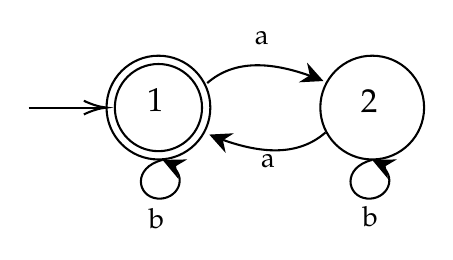
\begin{tikzpicture}[x=0.75pt,y=0.75pt,yscale=-1,xscale=1]
%uncomment if require: \path (0,118); %set diagram left start at 0, and has height of 118

%Shape: Circle [id:dp2043316806354638] 
\draw   (59,41) .. controls (59,27.19) and (70.19,16) .. (84,16) .. controls (97.81,16) and (109,27.19) .. (109,41) .. controls (109,54.81) and (97.81,66) .. (84,66) .. controls (70.19,66) and (59,54.81) .. (59,41) -- cycle ;
%Shape: Circle [id:dp8874779413660507] 
\draw   (162,41) .. controls (162,27.19) and (173.19,16) .. (187,16) .. controls (200.81,16) and (212,27.19) .. (212,41) .. controls (212,54.81) and (200.81,66) .. (187,66) .. controls (173.19,66) and (162,54.81) .. (162,41) -- cycle ;
%Straight Lines [id:da7500344624222353] 
\draw    (21.5,41) -- (57,41) ;
\draw [shift={(59,41)}, rotate = 180] [color={rgb, 255:red, 0; green, 0; blue, 0 }  ][line width=0.75]    (10.93,-3.29) .. controls (6.95,-1.4) and (3.31,-0.3) .. (0,0) .. controls (3.31,0.3) and (6.95,1.4) .. (10.93,3.29)   ;
%Curve Lines [id:da5093094901819417] 
\draw    (85.98,66.22) .. controls (71.48,69.82) and (73.48,83.82) .. (83.48,84.82) .. controls (92.83,85.76) and (99.56,74.45) .. (88.54,67.59) ;
\draw [shift={(85.98,66.22)}, rotate = 384.47] [fill={rgb, 255:red, 0; green, 0; blue, 0 }  ][line width=0.08]  [draw opacity=0] (10.72,-5.15) -- (0,0) -- (10.72,5.15) -- (7.12,0) -- cycle    ;
%Curve Lines [id:da27646448424610726] 
\draw    (186.98,66.22) .. controls (172.48,69.82) and (174.48,83.82) .. (184.48,84.82) .. controls (193.83,85.76) and (200.56,74.45) .. (189.54,67.59) ;
\draw [shift={(186.98,66.22)}, rotate = 384.47] [fill={rgb, 255:red, 0; green, 0; blue, 0 }  ][line width=0.08]  [draw opacity=0] (10.72,-5.15) -- (0,0) -- (10.72,5.15) -- (7.12,0) -- cycle    ;
%Shape: Circle [id:dp5930196324518537] 
\draw   (63,41) .. controls (63,29.4) and (72.4,20) .. (84,20) .. controls (95.6,20) and (105,29.4) .. (105,41) .. controls (105,52.6) and (95.6,62) .. (84,62) .. controls (72.4,62) and (63,52.6) .. (63,41) -- cycle ;
%Curve Lines [id:da5972834574265489] 
\draw    (107.5,29.2) .. controls (120.53,17.81) and (138.68,18.35) .. (161.05,27.2) ;
\draw [shift={(163.5,28.2)}, rotate = 202.64] [fill={rgb, 255:red, 0; green, 0; blue, 0 }  ][line width=0.08]  [draw opacity=0] (10.72,-5.15) -- (0,0) -- (10.72,5.15) -- (7.12,0) -- cycle    ;
%Curve Lines [id:da36846378229333165] 
\draw    (164.5,53) .. controls (151.47,64.39) and (133.32,63.85) .. (110.95,55) ;
\draw [shift={(108.5,54)}, rotate = 382.64] [fill={rgb, 255:red, 0; green, 0; blue, 0 }  ][line width=0.08]  [draw opacity=0] (10.72,-5.15) -- (0,0) -- (10.72,5.15) -- (7.12,0) -- cycle    ;

% Text Node
\draw (77,30) node [anchor=north west][inner sep=0.75pt]  [font=\large] [align=left] {1};
% Text Node
\draw (180,31) node [anchor=north west][inner sep=0.75pt]  [font=\large] [align=left] {2};
% Text Node
\draw (129,3) node [anchor=north west][inner sep=0.75pt]   [align=left] {a};
% Text Node
\draw (77.86,88.26) node [anchor=north west][inner sep=0.75pt]  [rotate=-359.87] [align=left] {b};
% Text Node
\draw (180.86,87.26) node [anchor=north west][inner sep=0.75pt]  [rotate=-359.87] [align=left] {b};
% Text Node
\draw (131.91,62.25) node [anchor=north west][inner sep=0.75pt]  [rotate=-359.38] [align=left] {a};


\end{tikzpicture}

\item



\tikzset{every picture/.style={line width=0.75pt}} %set default line width to 0.75pt        

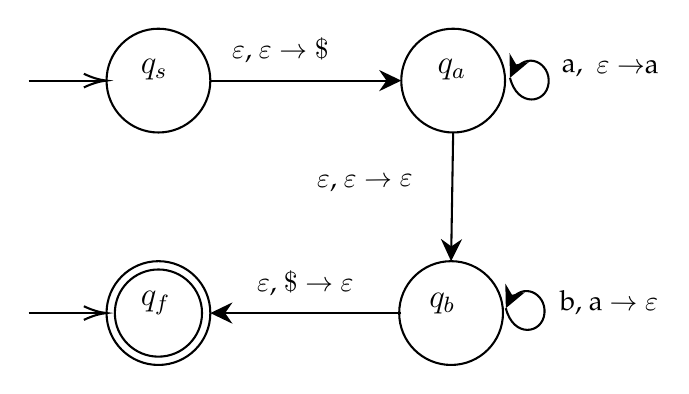
\begin{tikzpicture}[x=0.75pt,y=0.75pt,yscale=-1,xscale=1]
%uncomment if require: \path (0,199); %set diagram left start at 0, and has height of 199

%Shape: Circle [id:dp271471392298275] 
\draw   (53,44) .. controls (53,30.19) and (64.19,19) .. (78,19) .. controls (91.81,19) and (103,30.19) .. (103,44) .. controls (103,57.81) and (91.81,69) .. (78,69) .. controls (64.19,69) and (53,57.81) .. (53,44) -- cycle ;
%Shape: Circle [id:dp2021736081273684] 
\draw   (195,44) .. controls (195,30.19) and (206.19,19) .. (220,19) .. controls (233.81,19) and (245,30.19) .. (245,44) .. controls (245,57.81) and (233.81,69) .. (220,69) .. controls (206.19,69) and (195,57.81) .. (195,44) -- cycle ;
%Straight Lines [id:da9183350343495962] 
\draw    (15.5,44) -- (51,44) ;
\draw [shift={(53,44)}, rotate = 180] [color={rgb, 255:red, 0; green, 0; blue, 0 }  ][line width=0.75]    (10.93,-3.29) .. controls (6.95,-1.4) and (3.31,-0.3) .. (0,0) .. controls (3.31,0.3) and (6.95,1.4) .. (10.93,3.29)   ;
%Straight Lines [id:da5231631236234733] 
\draw    (103,44) -- (192,44) ;
\draw [shift={(195,44)}, rotate = 180] [fill={rgb, 255:red, 0; green, 0; blue, 0 }  ][line width=0.08]  [draw opacity=0] (10.72,-5.15) -- (0,0) -- (10.72,5.15) -- (7.12,0) -- cycle    ;
%Shape: Circle [id:dp9096213011848975] 
\draw   (194,156) .. controls (194,142.19) and (205.19,131) .. (219,131) .. controls (232.81,131) and (244,142.19) .. (244,156) .. controls (244,169.81) and (232.81,181) .. (219,181) .. controls (205.19,181) and (194,169.81) .. (194,156) -- cycle ;
%Curve Lines [id:da38257827769801] 
\draw    (247.38,42.66) .. controls (250.98,57.16) and (264.98,55.16) .. (265.98,45.16) .. controls (266.91,35.81) and (255.61,29.08) .. (248.74,40.1) ;
\draw [shift={(247.38,42.66)}, rotate = 294.47] [fill={rgb, 255:red, 0; green, 0; blue, 0 }  ][line width=0.08]  [draw opacity=0] (10.72,-5.15) -- (0,0) -- (10.72,5.15) -- (7.12,0) -- cycle    ;
%Straight Lines [id:da3592904350735662] 
\draw    (220,69) -- (219.05,128) ;
\draw [shift={(219,131)}, rotate = 270.92] [fill={rgb, 255:red, 0; green, 0; blue, 0 }  ][line width=0.08]  [draw opacity=0] (10.72,-5.15) -- (0,0) -- (10.72,5.15) -- (7.12,0) -- cycle    ;
%Curve Lines [id:da5279994650802105] 
\draw    (245.38,153.66) .. controls (248.98,168.16) and (262.98,166.16) .. (263.98,156.16) .. controls (264.91,146.81) and (253.61,140.08) .. (246.74,151.1) ;
\draw [shift={(245.38,153.66)}, rotate = 294.47] [fill={rgb, 255:red, 0; green, 0; blue, 0 }  ][line width=0.08]  [draw opacity=0] (10.72,-5.15) -- (0,0) -- (10.72,5.15) -- (7.12,0) -- cycle    ;
%Shape: Circle [id:dp6209857835409796] 
\draw   (53,156) .. controls (53,142.19) and (64.19,131) .. (78,131) .. controls (91.81,131) and (103,142.19) .. (103,156) .. controls (103,169.81) and (91.81,181) .. (78,181) .. controls (64.19,181) and (53,169.81) .. (53,156) -- cycle ;
%Straight Lines [id:da4734527758417679] 
\draw    (15.5,156) -- (51,156) ;
\draw [shift={(53,156)}, rotate = 180] [color={rgb, 255:red, 0; green, 0; blue, 0 }  ][line width=0.75]    (10.93,-3.29) .. controls (6.95,-1.4) and (3.31,-0.3) .. (0,0) .. controls (3.31,0.3) and (6.95,1.4) .. (10.93,3.29)   ;
%Straight Lines [id:da5459090974402354] 
\draw    (195,156) -- (106,156) ;
\draw [shift={(103,156)}, rotate = 360] [fill={rgb, 255:red, 0; green, 0; blue, 0 }  ][line width=0.08]  [draw opacity=0] (10.72,-5.15) -- (0,0) -- (10.72,5.15) -- (7.12,0) -- cycle    ;
%Shape: Circle [id:dp17662574233262274] 
\draw   (57,156) .. controls (57,144.4) and (66.4,135) .. (78,135) .. controls (89.6,135) and (99,144.4) .. (99,156) .. controls (99,167.6) and (89.6,177) .. (78,177) .. controls (66.4,177) and (57,167.6) .. (57,156) -- cycle ;

% Text Node
\draw (68,32) node [anchor=north west][inner sep=0.75pt]  [font=\large] [align=left] {$\displaystyle q_{s}$};
% Text Node
\draw (211,32) node [anchor=north west][inner sep=0.75pt]  [font=\large] [align=left] {$\displaystyle q_{a}$};
% Text Node
\draw (112,22) node [anchor=north west][inner sep=0.75pt]   [align=left] {$\displaystyle \varepsilon $, $\displaystyle \varepsilon \rightarrow \$$};
% Text Node
\draw (152.89,88.35) node [anchor=north west][inner sep=0.75pt]  [rotate=-359.31] [align=left] {$\displaystyle \varepsilon $, $\displaystyle \varepsilon \rightarrow \varepsilon $};
% Text Node
\draw (207,145) node [anchor=north west][inner sep=0.75pt]  [font=\large] [align=left] {$\displaystyle q_{b}$};
% Text Node
\draw (270.98,32.41) node [anchor=north west][inner sep=0.75pt]  [rotate=-0.45] [align=left] {a, \ $\displaystyle \varepsilon \rightarrow $a};
% Text Node
\draw (270,143.35) node [anchor=north west][inner sep=0.75pt]  [rotate=-0.58] [align=left] {b, a $\displaystyle \rightarrow \varepsilon $};
% Text Node
\draw (68,144) node [anchor=north west][inner sep=0.75pt]  [font=\large] [align=left] {$\displaystyle q_{f}$};
% Text Node
\draw (124,134) node [anchor=north west][inner sep=0.75pt]   [align=left] {$\displaystyle \varepsilon $, $\displaystyle \$\rightarrow \varepsilon $};


\end{tikzpicture}


\item



\tikzset{every picture/.style={line width=0.75pt}} %set default line width to 0.75pt        

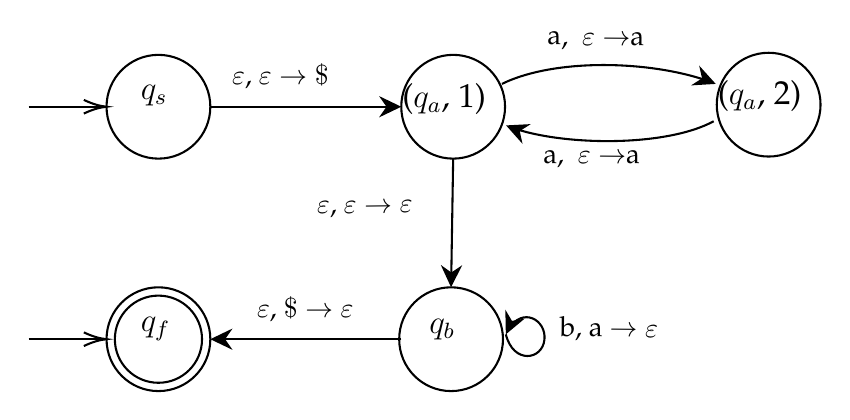
\begin{tikzpicture}[x=0.75pt,y=0.75pt,yscale=-1,xscale=1]
%uncomment if require: \path (0,195); %set diagram left start at 0, and has height of 195

%Shape: Circle [id:dp7426794074341168] 
\draw   (55,41) .. controls (55,27.19) and (66.19,16) .. (80,16) .. controls (93.81,16) and (105,27.19) .. (105,41) .. controls (105,54.81) and (93.81,66) .. (80,66) .. controls (66.19,66) and (55,54.81) .. (55,41) -- cycle ;
%Shape: Circle [id:dp5134913920036381] 
\draw   (197,41) .. controls (197,27.19) and (208.19,16) .. (222,16) .. controls (235.81,16) and (247,27.19) .. (247,41) .. controls (247,54.81) and (235.81,66) .. (222,66) .. controls (208.19,66) and (197,54.81) .. (197,41) -- cycle ;
%Straight Lines [id:da7528778304850927] 
\draw    (17.5,41) -- (53,41) ;
\draw [shift={(55,41)}, rotate = 180] [color={rgb, 255:red, 0; green, 0; blue, 0 }  ][line width=0.75]    (10.93,-3.29) .. controls (6.95,-1.4) and (3.31,-0.3) .. (0,0) .. controls (3.31,0.3) and (6.95,1.4) .. (10.93,3.29)   ;
%Straight Lines [id:da5982144898371642] 
\draw    (105,41) -- (194,41) ;
\draw [shift={(197,41)}, rotate = 180] [fill={rgb, 255:red, 0; green, 0; blue, 0 }  ][line width=0.08]  [draw opacity=0] (10.72,-5.15) -- (0,0) -- (10.72,5.15) -- (7.12,0) -- cycle    ;
%Shape: Circle [id:dp7675560256005667] 
\draw   (196,153) .. controls (196,139.19) and (207.19,128) .. (221,128) .. controls (234.81,128) and (246,139.19) .. (246,153) .. controls (246,166.81) and (234.81,178) .. (221,178) .. controls (207.19,178) and (196,166.81) .. (196,153) -- cycle ;
%Straight Lines [id:da8113476277012659] 
\draw    (222,66) -- (221.05,125) ;
\draw [shift={(221,128)}, rotate = 270.92] [fill={rgb, 255:red, 0; green, 0; blue, 0 }  ][line width=0.08]  [draw opacity=0] (10.72,-5.15) -- (0,0) -- (10.72,5.15) -- (7.12,0) -- cycle    ;
%Curve Lines [id:da1765096010716627] 
\draw    (247.38,150.66) .. controls (250.98,165.16) and (264.98,163.16) .. (265.98,153.16) .. controls (266.91,143.81) and (255.61,137.08) .. (248.74,148.1) ;
\draw [shift={(247.38,150.66)}, rotate = 294.47] [fill={rgb, 255:red, 0; green, 0; blue, 0 }  ][line width=0.08]  [draw opacity=0] (10.72,-5.15) -- (0,0) -- (10.72,5.15) -- (7.12,0) -- cycle    ;
%Shape: Circle [id:dp2431765631106455] 
\draw   (55,153) .. controls (55,139.19) and (66.19,128) .. (80,128) .. controls (93.81,128) and (105,139.19) .. (105,153) .. controls (105,166.81) and (93.81,178) .. (80,178) .. controls (66.19,178) and (55,166.81) .. (55,153) -- cycle ;
%Straight Lines [id:da6584667842801419] 
\draw    (17.5,153) -- (53,153) ;
\draw [shift={(55,153)}, rotate = 180] [color={rgb, 255:red, 0; green, 0; blue, 0 }  ][line width=0.75]    (10.93,-3.29) .. controls (6.95,-1.4) and (3.31,-0.3) .. (0,0) .. controls (3.31,0.3) and (6.95,1.4) .. (10.93,3.29)   ;
%Straight Lines [id:da2504818247658571] 
\draw    (197,153) -- (108,153) ;
\draw [shift={(105,153)}, rotate = 360] [fill={rgb, 255:red, 0; green, 0; blue, 0 }  ][line width=0.08]  [draw opacity=0] (10.72,-5.15) -- (0,0) -- (10.72,5.15) -- (7.12,0) -- cycle    ;
%Shape: Circle [id:dp2641274533588944] 
\draw   (59,153) .. controls (59,141.4) and (68.4,132) .. (80,132) .. controls (91.6,132) and (101,141.4) .. (101,153) .. controls (101,164.6) and (91.6,174) .. (80,174) .. controls (68.4,174) and (59,164.6) .. (59,153) -- cycle ;
%Shape: Circle [id:dp43430617190776877] 
\draw   (349,40) .. controls (349,26.19) and (360.19,15) .. (374,15) .. controls (387.81,15) and (399,26.19) .. (399,40) .. controls (399,53.81) and (387.81,65) .. (374,65) .. controls (360.19,65) and (349,53.81) .. (349,40) -- cycle ;
%Curve Lines [id:da9818578654645542] 
\draw    (245.5,30) .. controls (271.69,17.2) and (318.58,18.88) .. (346.01,29.03) ;
\draw [shift={(348.5,30)}, rotate = 202.17000000000002] [fill={rgb, 255:red, 0; green, 0; blue, 0 }  ][line width=0.08]  [draw opacity=0] (10.72,-5.15) -- (0,0) -- (10.72,5.15) -- (7.12,0) -- cycle    ;
%Curve Lines [id:da7573623733818997] 
\draw    (347.5,48) .. controls (324.34,60.55) and (274.64,59.87) .. (250.07,51) ;
\draw [shift={(247.5,50)}, rotate = 382.64] [fill={rgb, 255:red, 0; green, 0; blue, 0 }  ][line width=0.08]  [draw opacity=0] (10.72,-5.15) -- (0,0) -- (10.72,5.15) -- (7.12,0) -- cycle    ;

% Text Node
\draw (70,29) node [anchor=north west][inner sep=0.75pt]  [font=\large] [align=left] {$\displaystyle q_{s}$};
% Text Node
\draw (196,28) node [anchor=north west][inner sep=0.75pt]  [font=\large] [align=left] {($\displaystyle q_{a}$, 1)};
% Text Node
\draw (114,19) node [anchor=north west][inner sep=0.75pt]   [align=left] {$\displaystyle \varepsilon $, $\displaystyle \varepsilon \rightarrow \$$};
% Text Node
\draw (154.89,85.35) node [anchor=north west][inner sep=0.75pt]  [rotate=-359.31] [align=left] {$\displaystyle \varepsilon $, $\displaystyle \varepsilon \rightarrow \varepsilon $};
% Text Node
\draw (209,142) node [anchor=north west][inner sep=0.75pt]  [font=\large] [align=left] {$\displaystyle q_{b}$};
% Text Node
\draw (265.98,3.41) node [anchor=north west][inner sep=0.75pt]  [rotate=-0.45] [align=left] {a, \ $\displaystyle \varepsilon \rightarrow $a};
% Text Node
\draw (272,140.35) node [anchor=north west][inner sep=0.75pt]  [rotate=-0.58] [align=left] {b, a $\displaystyle \rightarrow \varepsilon $};
% Text Node
\draw (70,141) node [anchor=north west][inner sep=0.75pt]  [font=\large] [align=left] {$\displaystyle q_{f}$};
% Text Node
\draw (126,131) node [anchor=north west][inner sep=0.75pt]   [align=left] {$\displaystyle \varepsilon $, $\displaystyle \$\rightarrow \varepsilon $};
% Text Node
\draw (263.98,60.41) node [anchor=north west][inner sep=0.75pt]  [rotate=-0.45] [align=left] {a, \ $\displaystyle \varepsilon \rightarrow $a};
% Text Node
\draw (348,27) node [anchor=north west][inner sep=0.75pt]  [font=\large] [align=left] {($\displaystyle q_{a}$, 2)};


\end{tikzpicture}

\end{enumerate}

\newpage

\begin{prob}\end{prob}

\begin{enumerate}[label=(\alph*)]

\item

$L_1 = \{a^n b^m \pipe n \leq m\}$ can be concatenated with $L_2 = \{b\}$ to form $L_3 = \{a^n b^m \pipe n < m\}$. 
By closure properties, $L_1$ and $L_2$ are context-free, so $L_3$ must be as well. A similar argument 
can be made for $\{a^n b^m \pipe n > m\}$, except by concatenating $\{a\}$ instead.

\item

If we let $L_1 = \{a^n b^m \pipe n < m\}$, and $L_2 = \{a^n b^m \pipe n > m\}$
$L = \{a, b\}^* - \{a^n b^n \pipe n \in \N\}$ can be expressed as 
$ L_1^* \cup L_2^* \cup (L_1^R)^* \cup (L_2^R)^* $. 
Union, Reveseral, and Star are closed under context-free languages, 
so $L$ must also be context-free.

\end{enumerate}

\begin{prob}\end{prob}

\begin{enumerate}[label=(\alph*)]

\item
If we suppose that $L = \{a^n b a^n b a^n b \pipe n \geq 1 \}$ is context-free,
then we can assume some pumping length $p$. Suppose we have $w = a^{p-1} b a^{p-1} b a^{p - 1} b$.
The pumping lemma shows that we can construct $w$ as $uvxyz$, such that $|xyv| \leq p$ and
$v \neq \varepsilon$ or $y \neq varepsilon$. No matter what we pick for $v$ and $y$, pumping
those $v$ or $y$ will result in a word that is not in $L$. If either $v$ or $y$ is 
$\varepsilon$, letting the other select a substring in $w$, the largest substring that 
the other can be is $a^{p-1}b$ or $ba^{p-1}$, which if pumped, will result in an imbalance 
in the number of $a$s. If we have values for both $v$ and $y$, we still 
run into an issue, because there will always be a third set of $a$s that is
not being pumped. Therefore, $L$ is not context-free.

\item
We can use a regular language such as $aa*baa*baa*b$. $L \cap aa*baa*baa*b = \{a^n b a^n b a^n b \pipe n \geq 1\}$.
We already know that the right hand side is not context-free, which means $L$ cannot be context-free.

\end{enumerate}

\end{document}
